\subsectionaddtolist{طراحی سناریوی دوم}

مانند بخش قبل تمامی اجرا را با استفاده از کابل \lr{‫‪cooper straight-through‬‬‬} به هم وصل می‌کنیم. اما در اتصال دو روتر به هم نیاز است که از کابل \lr{serial ‫‪DCE‬‬} استفاده شود پس با خاموش کردن روترها ماژول \lr{WIC-1T} را به آنها اضافه می‌کنیم. 
\begin{figure}[h]
    \centering
    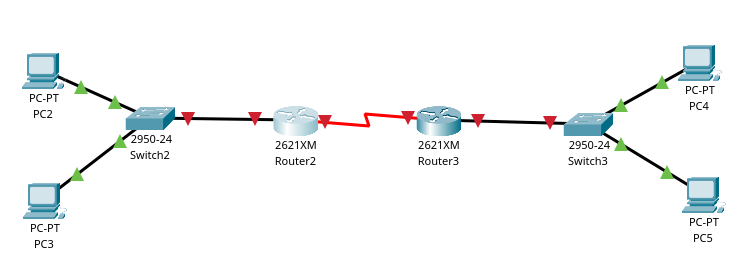
\includegraphics[width=1\textwidth]{img/12.png}
\end{figure}
\begin{figure}[h]
    \centering
    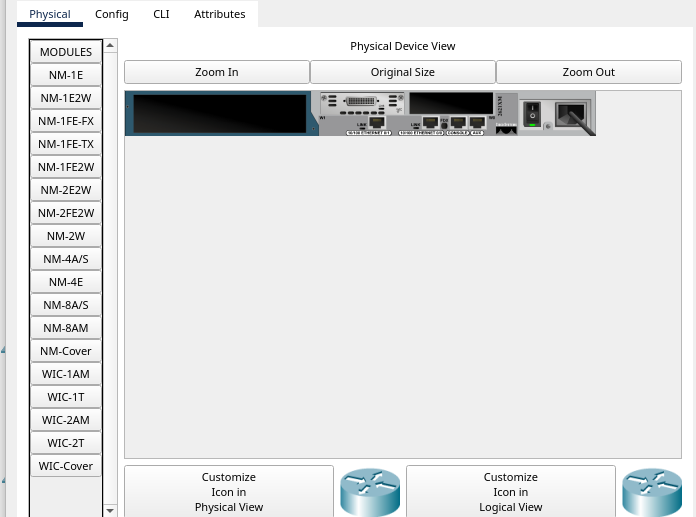
\includegraphics[width=1\textwidth]{img/11.png}
\end{figure}

برای اینکه اتصال بین دو روتر برقرار شود باید طبق فیلم با کلیک بر روی روترها در بخش config و در \lr{serial 0/0} مقدار کلاک را به 56000 تغییر دهیم و گزینه on را فعال کنیم.
\begin{figure}[h]
    \centering
    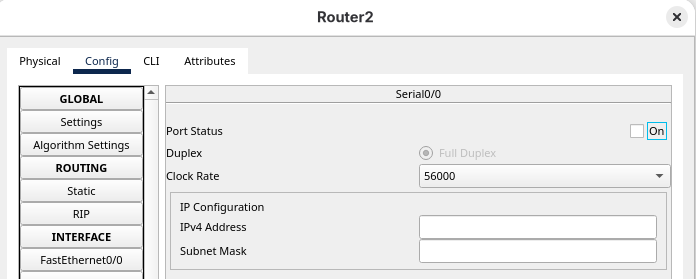
\includegraphics[width=1\textwidth]{img/14.png}
    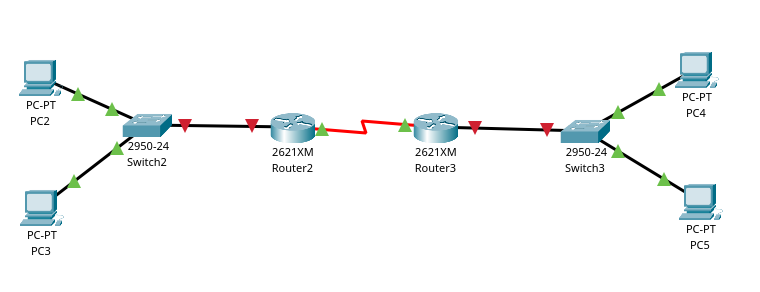
\includegraphics[width=1\textwidth]{img/13.png}
\end{figure}
\clearpage
حال مانند بخش قبل به پیکربندی اجزا می‌پردازیم.

\begin{figure}[h]
    \centering
    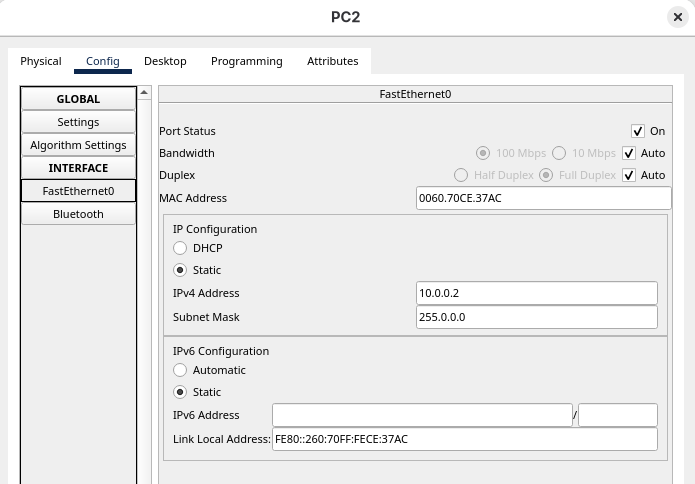
\includegraphics[width=1\textwidth]{img/15.png}
\end{figure}
\begin{figure}[h]
    \centering
    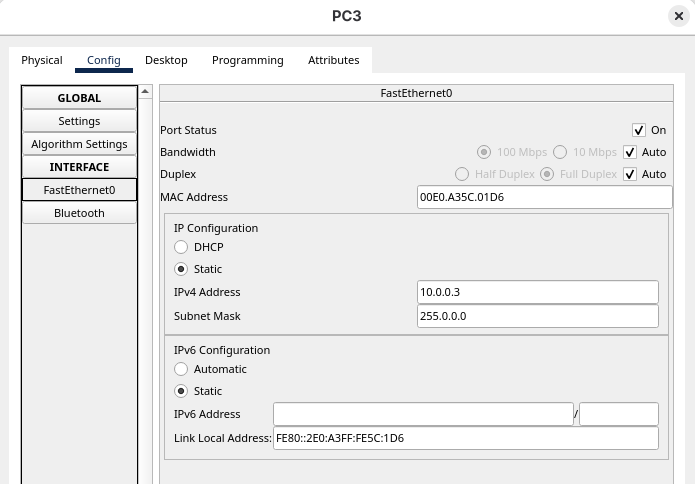
\includegraphics[width=1\textwidth]{img/16.png}
\end{figure}
\begin{figure}[h]
    \centering
    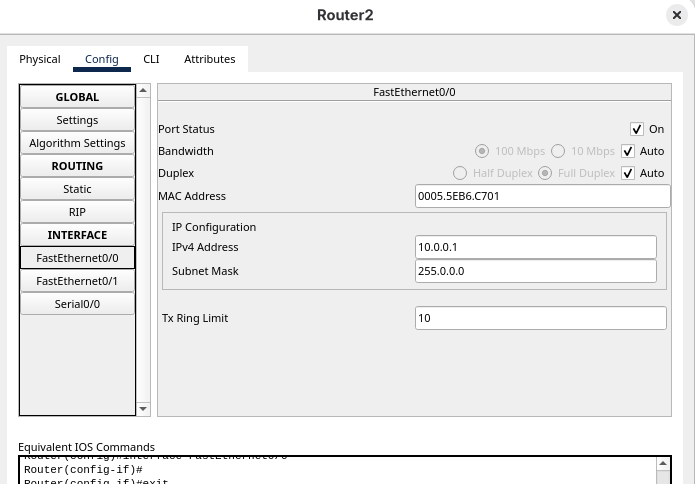
\includegraphics[width=1\textwidth]{img/17.png}
\end{figure}
\begin{figure}[h]
    \centering
    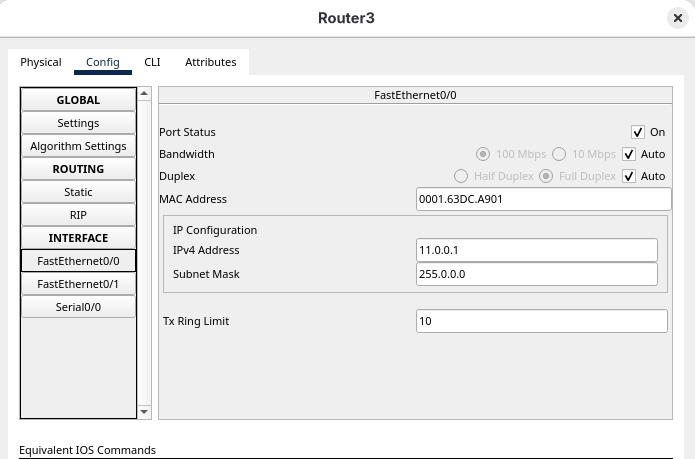
\includegraphics[width=1\textwidth]{img/18.png}
\end{figure}
\begin{figure}[h]
    \centering
    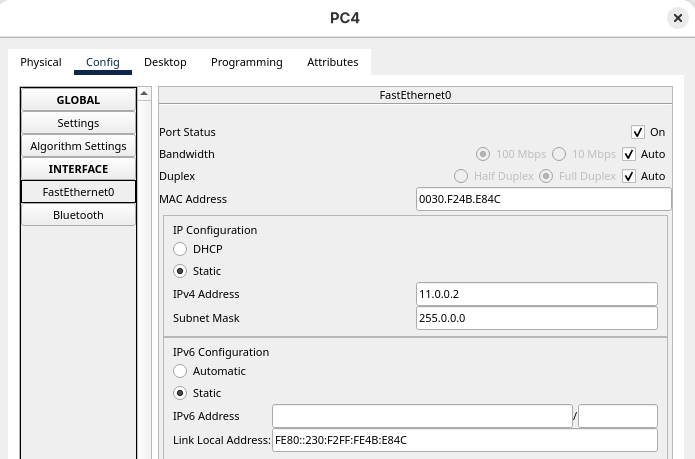
\includegraphics[width=1\textwidth]{img/19.png}
\end{figure}
\begin{figure}[h]
    \centering
    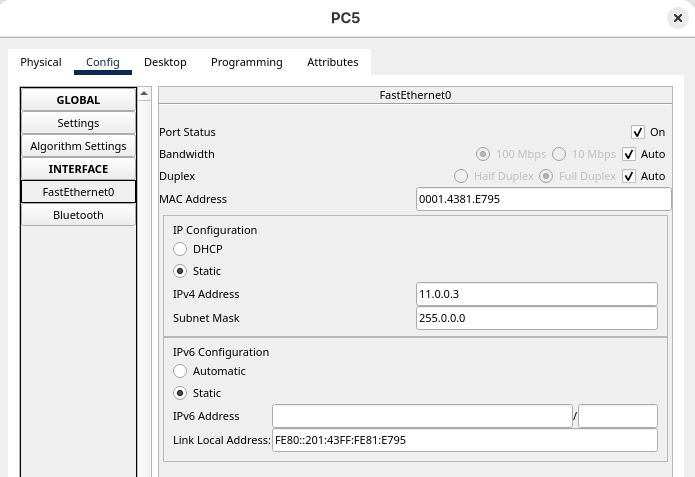
\includegraphics[width=1\textwidth]{img/20.png}
\end{figure}
\begin{figure}[h]
    \centering
    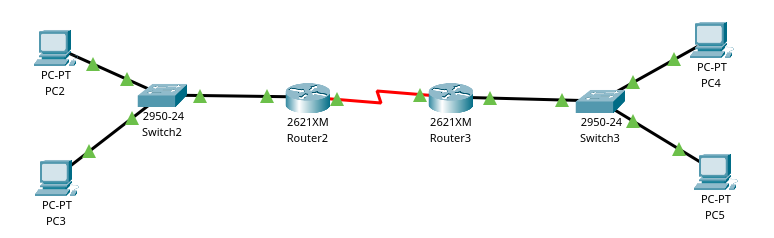
\includegraphics[width=1\textwidth]{img/21.png}
\end{figure}

\clearpage
تا الان اتصال بین کامپیوترها با سوئیچ مشترک برقرار است اما طبق فیلم برای اینکه روترها را هم بشناسیم باید یک subnet بین آنها تعریف شود. 
\begin{figure}[h]
    \centering
    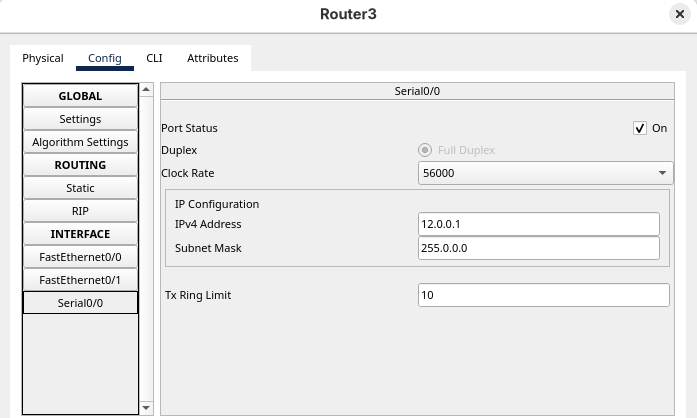
\includegraphics[width=1\textwidth]{img/22.png}
\end{figure}
\begin{figure}[h]
    \centering
    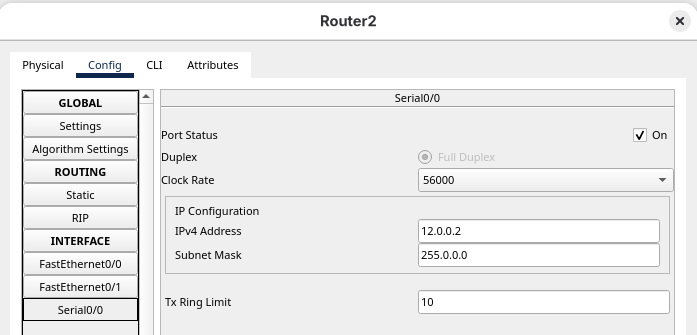
\includegraphics[width=1\textwidth]{img/23.png}
\end{figure}
\\
حال باید روترها بتوانند subnet دیگری را از طریق لینک داده شده عبور دهد. برای اینکار در بخش config در منوی static آی‌پی‌های مجاز را وارد می‌کنیم.
\begin{figure}[h]
    \centering
    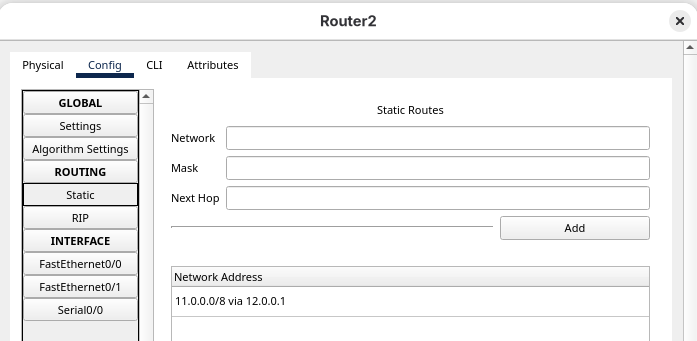
\includegraphics[width=1\textwidth]{img/26.png}
    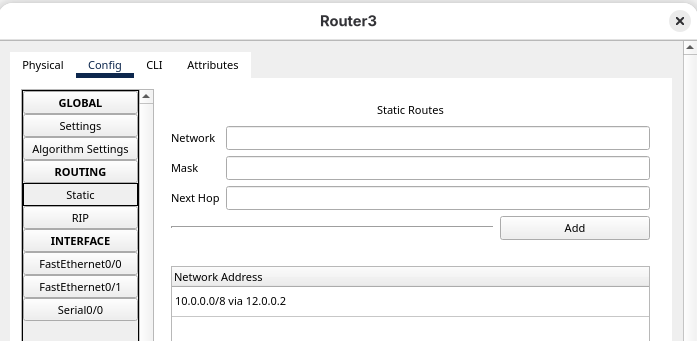
\includegraphics[width=1\textwidth]{img/27.png}
\end{figure}

\clearpage
برای تست مانند بخش قبل بین کامپیوترها از دستور پینگ استفاده می‌کنیم.
\begin{figure}[h]
    \centering
    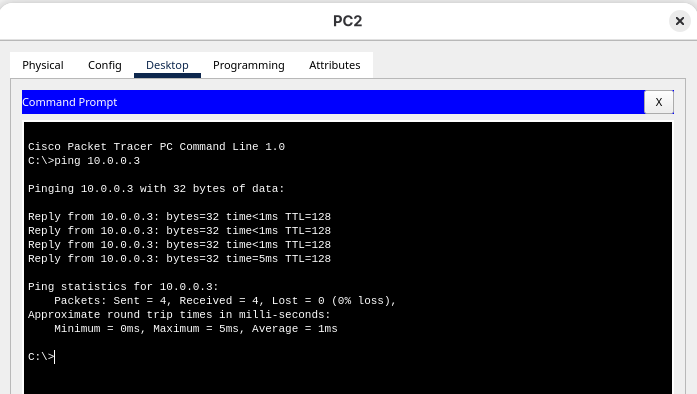
\includegraphics[width=1\textwidth]{img/24.png}
    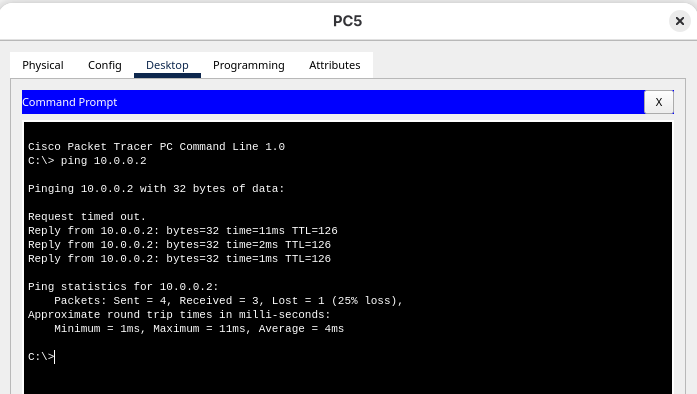
\includegraphics[width=1\textwidth]{img/25.png}
\end{figure}

